\documentclass[conference]{IEEEtran}
\IEEEoverridecommandlockouts
% The preceding line is only needed to identify funding in the first footnote. If that is unneeded, please comment it out.
\usepackage{cite}
\usepackage{amsmath,amssymb,amsfonts}
\usepackage{algorithmic}
\usepackage{graphicx}
\usepackage{textcomp}
\usepackage{xcolor}
\usepackage{url}
\usepackage[section]{placeins}
\usepackage[nobottomtitles]{titlesec}
\def\BibTeX{{\rm B\kern-.05em{\sc i\kern-.025em b}\kern-.08em
    T\kern-.1667em\lower.7ex\hbox{E}\kern-.125emX}}
\begin{document}
\graphicspath{ {./images/} }

\title{Web-based IoT Dashboard and Analytics\\}

\author{\IEEEauthorblockN{MUHAMMAD AIDIL SYAZWAN BIN HAMDAN}
(Student)\\
\IEEEauthorblockA{\textit{FACULTY OF COMPUTING} \\
UNIVERSITY MALAYSIA PAHANG\\
26600, PEKAN, KUANTAN, PAHANG \\
Email: th3ygen@gmail.com}
\and
\IEEEauthorblockN{Dr. SYAFIQ FAUZI BIN KAMARULZAMAN}
(Supervisor)\\
\IEEEauthorblockA{\textit{FACULTY OF COMPUTING} \\
UNIVERSITY MALAYSIA PAHANG\\
26600, PEKAN, KUANTAN, PAHANG \\
Email: syafiq29@ump.edu.my}
}

\maketitle

\begin{IEEEkeywords}
iot, machine-to-machine, m2m, big data, data analytics, data dashboard, data visualization
\end{IEEEkeywords}

\section{Introduction}

\subsection{Background}
The Internet of Things (IoT) refers to a system of interrelated, internet-connected objects
that are able to collect and transfer data over a wireless network without human intervention
\cite{b1}. The concept of IoT has been around for a long time and it has contributed a significant
impact on the development of world technology. Nowadays, almost everything around us is an
IoT device such as smartwatch, home security system, and even the famous voice assistant,
Alexa, is an IoT device. In short, any physical device that is accessible thru the Internet,
exchanges information between other devices, and does not require human intervention is
considered an IoT device. According to the statistics, throughout the year since the first
day of the IoT era, total things connected are increasing drastically. In 2016, total things
connected are roughly around 4.7 billion, then in 2021, the number reached a total of
11.6 billion of IoT devices \cite{b2}. Going back to the project title, IoT dashboard is the
graphical presentation of IoT device data.

An IoT dashboard is basically an IoT control panel that can achieve many different goals for
any business \cite{b3}. It emphasises the capability of pulling data from remote IoT devices and
summarising them into meaningful information. Additionally, interprets the information into
simple and purposeful charts. What makes this system more robust is all of the processes
are in real-time. The dashboard is not limited to the system specifications, the charts
and the dashboard layout can be customized based on the researcher's needs. 

As the adoption of IoT in the industrial field exponentially increases, the data transmitted
from IoT devices especially from large scale projects grows larger and becomes incomprehensive
for humans to read. In addition, the IoT devices' status such as temperature and performance
needs to be monitored. It sounds easy, but when hundreds or thousands of IoT devices
are involved, things will get tedious. Thus, the use of an IoT dashboard along with
extra analytical features and functionalities needs to be considered.

\subsection{Problem statements}
Monitoring IoT data is crucial as it influences the performance and quality of a project 
or solution. In addition, the flexibility and robustness of the monitoring system should 
be considered to provide the best view of the IoT data that fits the researcher’s 
requirements. Most of the existing systems do not offer sufficient features such as 
data filtering that takes the data into a customizable equation. Furthermore, not many 
of the existing systems allow its user to utilize the full potential of an IoT dashboard 
system. Some systems limit the availability of graphical components of the data 
visualization while some do not provide the functionality to export the researching 
data into certain formats such as XLSX, JSON, CSV, XML, or as image file. 
Last but not least, sharing the research or dashboard to the public is not a 
common thing amongst the existing system. This feature is very important and 
useful as it creates the environment for the researchers to discuss or suggest 
for an improvement. With most analytical features and data functionalities included 
in the new solution, such problems can be countered.

\subsection{Scope}
The scope of the project are listed as below:
\begin{enumerate}
    \item The system is focused on researchers as its user which includes lecturers, students, and data analysts.
    \item The data for the IoT dashboard are from IoT devices only.
\end{enumerate}

\subsection{Objectives}
The project objectives are as listed below:
\begin{enumerate}
    \item To develop an IoT dashboard system with the best user experience in both user interface and functionalities.
    \item To design a system that is capable of applying custom equations for each data pulled from IoT devices.
    \item To provide the best environment for researchers to conduct public discussion regarding the IoT data.
\end{enumerate}

\section{Methodology}


\begin{figure}[h]
    \centering
    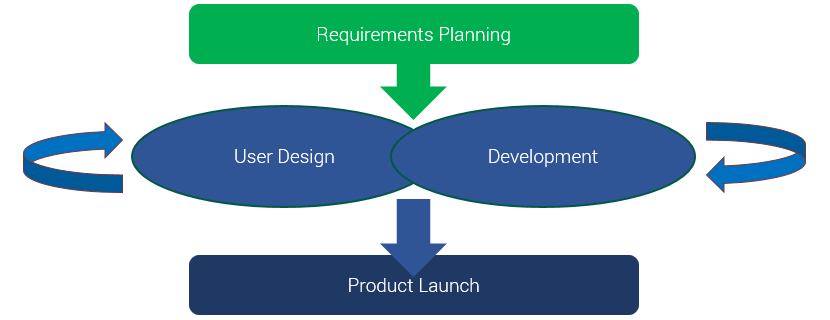
\includegraphics[width=0.35\textwidth]{rad}
    \caption{Rapid Development Model Scheme}
    \label{fig:rad}
\end{figure}

\FloatBarrier
As shown in figure \ref{fig:rad}, the project development will be based on the Rapid Development 
model. It consists of three major steps, starting with Requirement Planning. The first step 
of the development is the phase where requirements are in the main focus. Requirements for 
both functional and non-functional will be investigated based on the project scope and user 
needs. The next step will be the iterative phase that consists of two components, User Design 
and Development. For the User Design part, the looks, feel, functionality, and the user 
interface design of the system will be identified and drawn. This includes the charts and 
dashboard layout. Once it meets certain requirements, the illustrated User Design will go 
into the Development phase where it will be realized as part of the system. This process 
will be done consecutively until all of the requirements are met. Finally, the last phase 
which is Product Launch, is where the system will be deployed and delivered to the users. 
In this phase, the system is expected to be fully working based on the deliverables and the 
user should be able to monitor their IoT data as promised.

\section{Flowcharts}


\begin{figure}[h]
    \centering
    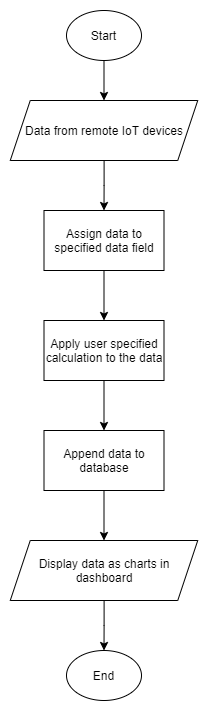
\includegraphics[height=0.45\textwidth]{flow}
    \caption{System flowchart}
    \label{fig:flow}
\end{figure}

\FloatBarrier

\section{Expected outcome}
\begin{figure}[h]
    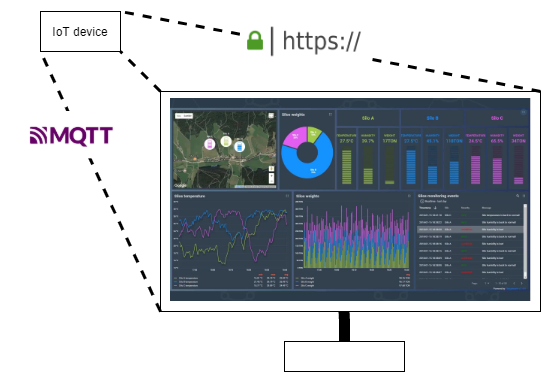
\includegraphics[width=0.4\textwidth]{outcome}
    \caption{Expected outcome}
    \label{fig:outcome}
\end{figure}

\section{Conclusion}
Summarising the project, IoT gives significant impacts in our daily life in numerous fields 
such as medical, security, and industrial. Not to forget that the current technology is 
revolving along The Fourth Industrial Revolution (4IR), IoT is one of the core components 
in achieving 4IR goals. 4IR refers to a new phase in the Industrial Revolution that focuses 
heavily on interconnectivity, automation, machine learning, and real-time data \cite{b4}. It is 
expected that in the future, IoT will be widely used in various sectors around the globe. 
Thus, with the early IoT dashboard development and improvements, it is considered as a 
stepping stone towards welcoming the new phase of Industrial Revolution.

\begin{thebibliography}{00}
\bibitem{b1} "What is IoT? Defining the Internet of Things (IoT)" [Online] Available: https://www.aeris.com/in/what-is-iot/

[Accessed: 16 April 2021]
\bibitem{b2} "Prediction 2021: Technology Trends that will drive IoT growth", February 6, 2021, [Online] Available: \url{https://www.europeanbusinessreview.com/prediction-2021-technology-trends-that-will-drive-iot-growth/#:~:text=From%20mere%204.7%20billion%20things,multi%2Dfolds%20in%20coming%20years.}

[Accessed: 16 April 2021]
\bibitem{b3} "How to Create Web Dashboards for IoT Devices", January 24 2020, [Online] Available: \url{https://www.mobindustry.net/how-to-create-web-dashboards-for-iot-devices/#:~:text=An%20IoT%20dashboard%20is%20web,Collect%20data%20from%20your%20devices.}

[Accessed: 16 April 2021]
\bibitem{b4} "What is Industry 4.0—the Industrial Internet of Things (IIoT)?" [Online] Available: \url{https://www.epicor.com/en-my/resource-center/articles/what-is-industry-4-0/}

[Accessed: 16 April 2021]
\end{thebibliography}
\vspace{12pt}

\end{document}